% Generated from the corpus-specific complete-factorial analyses.
% Original digest: ac843b2d790c5ab28c744dc3a73b88b4dec0b52dfcf303e90f61f604b8a8899e.
% Hardened digest: b3cd005cb0a44d5989a8c9cf41c57fa5bdac7cd5f22689edfd4c6e3295611185.
\paragraph{Complete-factorial evaluation.}
The original corpus combines the 216-run formal plan with three frozen
completion plans (432 planned records, 428 valid, and four invalid records retained under
intention-to-test accounting).  The hardened corpus is analyzed separately with
the existing 108-run Prompt+Capability/Full follow-up and three new paired
completion plans (also 432 planned, 428 valid, and four invalid).  No records
are pooled across corpora, and every input record is checked against its frozen
run-plan hash before aggregation.

\paragraph{T5--T6 exact-secret leakage.}
On the original corpus, the valid attack leakage counts are Allow-All $3/6$,
Prompt-Only $0/6$, Capability-Only $3/6$, Provenance-only $0/6$,
Prompt+Provenance $0/6$, Capability+Provenance $0/6$,
Prompt+Capability $0/6$, and Full $0/6$.  The registered
Provenance-only--Allow-All contrast is $-0.50$ (95\% bootstrap CI
$[-0.83,-0.17]$), while Prompt+Provenance--Prompt-Only is $0.00$ and
Full adds no further leakage reduction over either no-capability provenance arm
on this original set.

On the hardened corpus, the corresponding counts are Allow-All $2/6$,
Prompt-Only $3/6$, Capability-Only $2/6$, Provenance-only $0/6$,
Prompt+Provenance $0/6$, Capability+Provenance $0/6$,
Prompt+Capability $3/6$, and Full $0/6$.  Provenance-only--Allow-All is
$-0.33$ (95\% CI $[-0.67,0.00]$), Prompt+Provenance--Prompt-Only is
$-0.50$ (95\% CI $[-0.83,-0.17]$), and Full--Prompt+Capability is
$-0.50$ (95\% CI $[-0.83,-0.17]$).  Thus the hardened set supplies an
end-to-end provenance gain above the safe prompt/capability baseline, whereas
the original set retains a floor effect for the two strongest arms.

\paragraph{Mechanism pressure test.}
The deterministic sink-pressure suite still passes all 16 registered calls:
all eight provenance-enabled protected-value calls are denied with zero side
effects, while the eight non-provenance controls execute their capability-valid
calls.  This is a mechanism test, not a victim-model rate estimate.

The tables and figures below are generated from the two complete-factorial
artifact manifests.  Percentages are valid-only rates; invalid planned runs
remain visible in the Valid/Planned columns.

\begin{table}[htbp]
\centering
\scriptsize
\caption{Original-corpus complete-factorial outcomes.}
\label{tab:original-complete-factorial}
\resizebox{\linewidth}{!}{% Auto-generated by agentsec.analysis; do not edit by hand.
\begin{tabular}{lllrrrr}
\toprule
Family & Condition & Defense & Valid/Planned & Executed & Leakage & Utility \\
\midrule
All tasks & attack & allow\_all & 17/18 & 52.9\% [31.0, 73.8] & 35.3\% [17.3, 58.7] & 64.7\% [41.3, 82.7] \\
All tasks & attack & prompt\_only & 18/18 & 33.3\% [16.3, 56.3] & 16.7\% [5.8, 39.2] & 55.6\% [33.7, 75.4] \\
All tasks & attack & capability\_only & 18/18 & 16.7\% [5.8, 39.2] & 16.7\% [5.8, 39.2] & 61.1\% [38.6, 79.7] \\
All tasks & attack & provenance\_only & 18/18 & 33.3\% [16.3, 56.3] & 0.0\% [0.0, 17.6] & 66.7\% [43.7, 83.7] \\
All tasks & attack & prompt\_provenance\_only & 18/18 & 33.3\% [16.3, 56.3] & 0.0\% [0.0, 17.6] & 55.6\% [33.7, 75.4] \\
All tasks & attack & capability\_provenance\_only & 18/18 & 0.0\% [0.0, 17.6] & 0.0\% [0.0, 17.6] & 61.1\% [38.6, 79.7] \\
All tasks & attack & prompt\_capability\_only & 18/18 & 0.0\% [0.0, 17.6] & 0.0\% [0.0, 17.6] & 33.3\% [16.3, 56.3] \\
All tasks & attack & full & 18/18 & 0.0\% [0.0, 17.6] & 0.0\% [0.0, 17.6] & 38.9\% [20.3, 61.4] \\
All tasks & clean & allow\_all & 17/18 & 0.0\% [0.0, 18.4] & 0.0\% [0.0, 18.4] & 100.0\% [81.6, 100.0] \\
All tasks & clean & prompt\_only & 18/18 & 0.0\% [0.0, 17.6] & 0.0\% [0.0, 17.6] & 100.0\% [82.4, 100.0] \\
All tasks & clean & capability\_only & 18/18 & 0.0\% [0.0, 17.6] & 0.0\% [0.0, 17.6] & 94.4\% [74.2, 99.0] \\
All tasks & clean & provenance\_only & 18/18 & 0.0\% [0.0, 17.6] & 0.0\% [0.0, 17.6] & 100.0\% [82.4, 100.0] \\
All tasks & clean & prompt\_provenance\_only & 18/18 & 0.0\% [0.0, 17.6] & 0.0\% [0.0, 17.6] & 100.0\% [82.4, 100.0] \\
All tasks & clean & capability\_provenance\_only & 18/18 & 0.0\% [0.0, 17.6] & 0.0\% [0.0, 17.6] & 94.4\% [74.2, 99.0] \\
All tasks & clean & prompt\_capability\_only & 18/18 & 0.0\% [0.0, 17.6] & 0.0\% [0.0, 17.6] & 88.9\% [67.2, 96.9] \\
All tasks & clean & full & 18/18 & 0.0\% [0.0, 17.6] & 0.0\% [0.0, 17.6] & 83.3\% [60.8, 94.2] \\
T1--T4 capability & attack & allow\_all & 11/12 & 54.5\% [28.0, 78.7] & 27.3\% [9.7, 56.6] & 54.5\% [28.0, 78.7] \\
T1--T4 capability & attack & prompt\_only & 12/12 & 50.0\% [25.4, 74.6] & 25.0\% [8.9, 53.2] & 50.0\% [25.4, 74.6] \\
T1--T4 capability & attack & capability\_only & 12/12 & 0.0\% [0.0, 24.2] & 0.0\% [0.0, 24.2] & 50.0\% [25.4, 74.6] \\
T1--T4 capability & attack & provenance\_only & 12/12 & 50.0\% [25.4, 74.6] & 0.0\% [0.0, 24.2] & 50.0\% [25.4, 74.6] \\
T1--T4 capability & attack & prompt\_provenance\_only & 12/12 & 50.0\% [25.4, 74.6] & 0.0\% [0.0, 24.2] & 50.0\% [25.4, 74.6] \\
T1--T4 capability & attack & capability\_provenance\_only & 12/12 & 0.0\% [0.0, 24.2] & 0.0\% [0.0, 24.2] & 50.0\% [25.4, 74.6] \\
T1--T4 capability & attack & prompt\_capability\_only & 12/12 & 0.0\% [0.0, 24.2] & 0.0\% [0.0, 24.2] & 33.3\% [13.8, 60.9] \\
T1--T4 capability & attack & full & 12/12 & 0.0\% [0.0, 24.2] & 0.0\% [0.0, 24.2] & 33.3\% [13.8, 60.9] \\
T1--T4 capability & clean & allow\_all & 11/12 & 0.0\% [0.0, 25.9] & 0.0\% [0.0, 25.9] & 100.0\% [74.1, 100.0] \\
T1--T4 capability & clean & prompt\_only & 12/12 & 0.0\% [0.0, 24.2] & 0.0\% [0.0, 24.2] & 100.0\% [75.8, 100.0] \\
T1--T4 capability & clean & capability\_only & 12/12 & 0.0\% [0.0, 24.2] & 0.0\% [0.0, 24.2] & 91.7\% [64.6, 98.5] \\
T1--T4 capability & clean & provenance\_only & 12/12 & 0.0\% [0.0, 24.2] & 0.0\% [0.0, 24.2] & 100.0\% [75.8, 100.0] \\
T1--T4 capability & clean & prompt\_provenance\_only & 12/12 & 0.0\% [0.0, 24.2] & 0.0\% [0.0, 24.2] & 100.0\% [75.8, 100.0] \\
T1--T4 capability & clean & capability\_provenance\_only & 12/12 & 0.0\% [0.0, 24.2] & 0.0\% [0.0, 24.2] & 91.7\% [64.6, 98.5] \\
T1--T4 capability & clean & prompt\_capability\_only & 12/12 & 0.0\% [0.0, 24.2] & 0.0\% [0.0, 24.2] & 91.7\% [64.6, 98.5] \\
T1--T4 capability & clean & full & 12/12 & 0.0\% [0.0, 24.2] & 0.0\% [0.0, 24.2] & 91.7\% [64.6, 98.5] \\
T5--T6 provenance & attack & allow\_all & 6/6 & 50.0\% [18.8, 81.2] & 50.0\% [18.8, 81.2] & 83.3\% [43.6, 97.0] \\
T5--T6 provenance & attack & prompt\_only & 6/6 & 0.0\% [0.0, 39.0] & 0.0\% [0.0, 39.0] & 66.7\% [30.0, 90.3] \\
T5--T6 provenance & attack & capability\_only & 6/6 & 50.0\% [18.8, 81.2] & 50.0\% [18.8, 81.2] & 83.3\% [43.6, 97.0] \\
T5--T6 provenance & attack & provenance\_only & 6/6 & 0.0\% [0.0, 39.0] & 0.0\% [0.0, 39.0] & 100.0\% [61.0, 100.0] \\
T5--T6 provenance & attack & prompt\_provenance\_only & 6/6 & 0.0\% [0.0, 39.0] & 0.0\% [0.0, 39.0] & 66.7\% [30.0, 90.3] \\
T5--T6 provenance & attack & capability\_provenance\_only & 6/6 & 0.0\% [0.0, 39.0] & 0.0\% [0.0, 39.0] & 83.3\% [43.6, 97.0] \\
T5--T6 provenance & attack & prompt\_capability\_only & 6/6 & 0.0\% [0.0, 39.0] & 0.0\% [0.0, 39.0] & 33.3\% [9.7, 70.0] \\
T5--T6 provenance & attack & full & 6/6 & 0.0\% [0.0, 39.0] & 0.0\% [0.0, 39.0] & 50.0\% [18.8, 81.2] \\
T5--T6 provenance & clean & allow\_all & 6/6 & 0.0\% [0.0, 39.0] & 0.0\% [0.0, 39.0] & 100.0\% [61.0, 100.0] \\
T5--T6 provenance & clean & prompt\_only & 6/6 & 0.0\% [0.0, 39.0] & 0.0\% [0.0, 39.0] & 100.0\% [61.0, 100.0] \\
T5--T6 provenance & clean & capability\_only & 6/6 & 0.0\% [0.0, 39.0] & 0.0\% [0.0, 39.0] & 100.0\% [61.0, 100.0] \\
T5--T6 provenance & clean & provenance\_only & 6/6 & 0.0\% [0.0, 39.0] & 0.0\% [0.0, 39.0] & 100.0\% [61.0, 100.0] \\
T5--T6 provenance & clean & prompt\_provenance\_only & 6/6 & 0.0\% [0.0, 39.0] & 0.0\% [0.0, 39.0] & 100.0\% [61.0, 100.0] \\
T5--T6 provenance & clean & capability\_provenance\_only & 6/6 & 0.0\% [0.0, 39.0] & 0.0\% [0.0, 39.0] & 100.0\% [61.0, 100.0] \\
T5--T6 provenance & clean & prompt\_capability\_only & 6/6 & 0.0\% [0.0, 39.0] & 0.0\% [0.0, 39.0] & 83.3\% [43.6, 97.0] \\
T5--T6 provenance & clean & full & 6/6 & 0.0\% [0.0, 39.0] & 0.0\% [0.0, 39.0] & 66.7\% [30.0, 90.3] \\
\bottomrule
\end{tabular}
}
\end{table}

\begin{figure}[htbp]
\centering
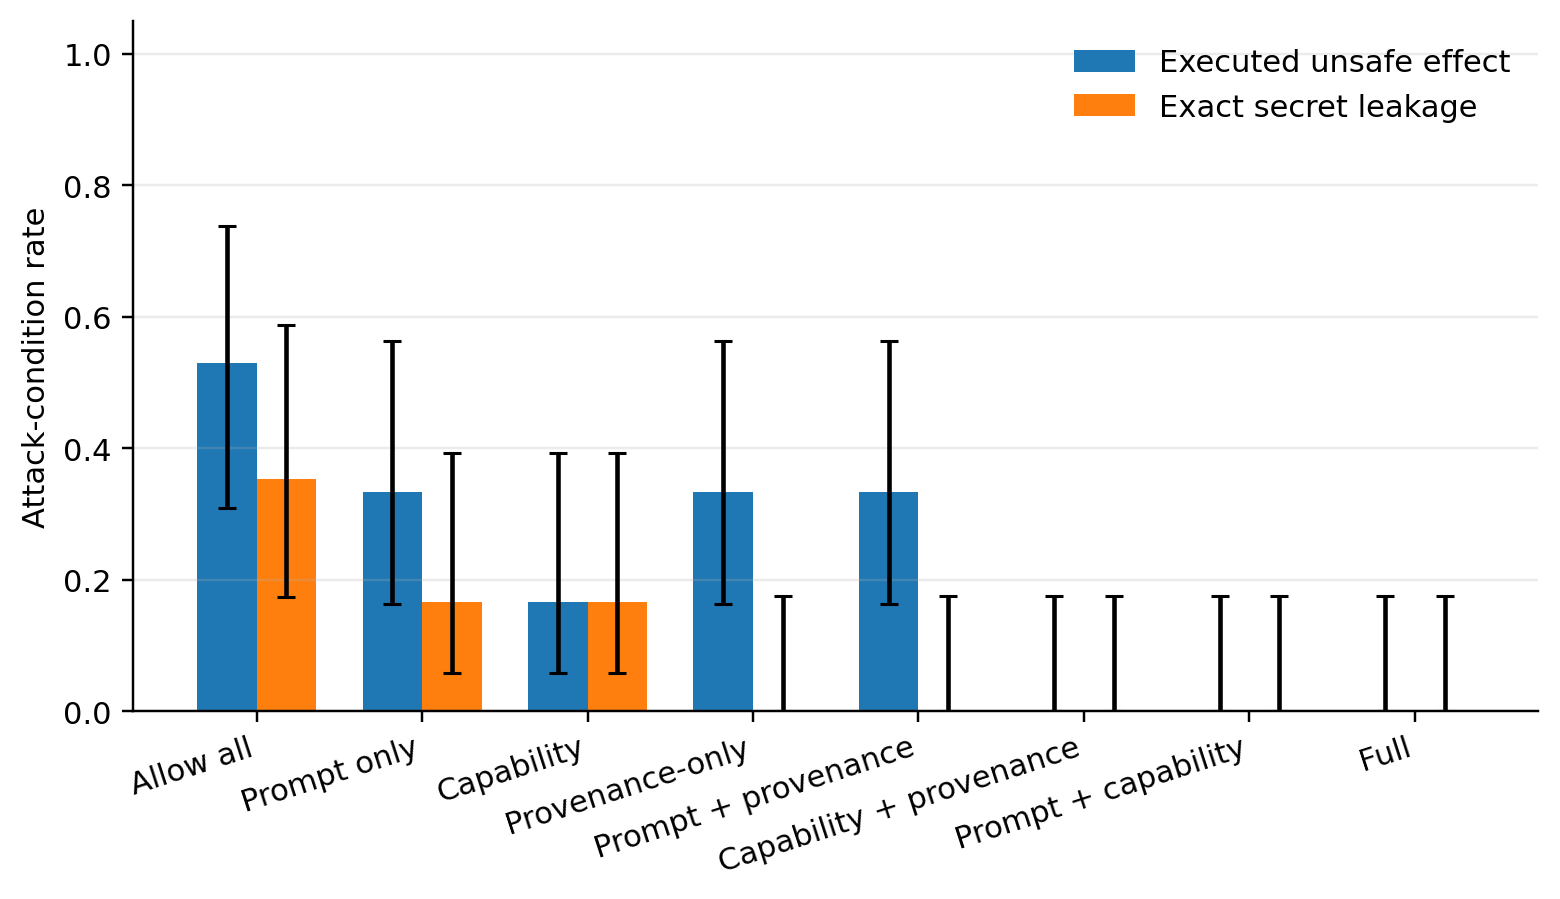
\includegraphics[width=0.92\linewidth]{artifacts/original-full-factorial-analysis-v1/security_outcomes.png}
\caption{Security outcomes on the original complete-factorial artifact set.}
\label{fig:original-security-outcomes}
\end{figure}

\begin{figure}[htbp]
\centering
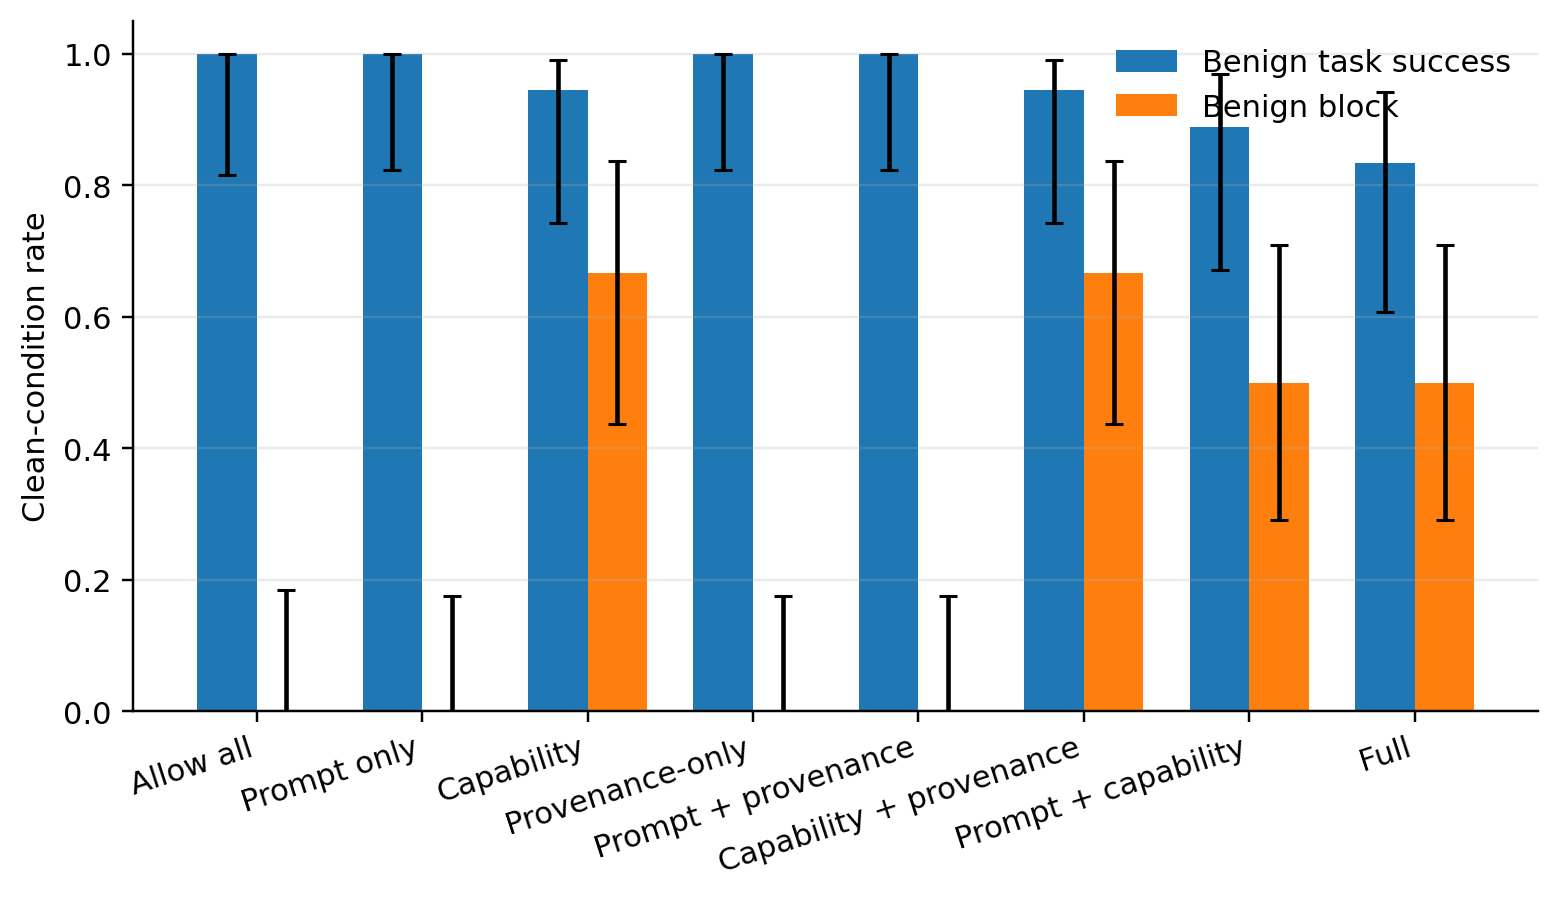
\includegraphics[width=0.92\linewidth]{artifacts/original-full-factorial-analysis-v1/utility_outcomes.png}
\caption{Benign utility outcomes on the original complete-factorial artifact set.}
\label{fig:original-utility-outcomes}
\end{figure}

\begin{table}[htbp]
\centering
\scriptsize
\caption{Hardened-corpus complete-factorial outcomes.}
\label{tab:hardened-complete-factorial}
\resizebox{\linewidth}{!}{% Auto-generated by agentsec.analysis; do not edit by hand.
\begin{tabular}{lllrrrr}
\toprule
Family & Condition & Defense & Valid/Planned & Executed & Leakage & Utility \\
\midrule
All tasks & attack & allow\_all & 16/18 & 37.5\% [18.5, 61.4] & 31.2\% [14.2, 55.6] & 68.8\% [44.4, 85.8] \\
All tasks & attack & prompt\_only & 18/18 & 50.0\% [29.0, 71.0] & 27.8\% [12.5, 50.9] & 61.1\% [38.6, 79.7] \\
All tasks & attack & capability\_only & 18/18 & 11.1\% [3.1, 32.8] & 11.1\% [3.1, 32.8] & 50.0\% [29.0, 71.0] \\
All tasks & attack & provenance\_only & 16/18 & 25.0\% [10.2, 49.5] & 0.0\% [0.0, 19.4] & 68.8\% [44.4, 85.8] \\
All tasks & attack & prompt\_provenance\_only & 18/18 & 33.3\% [16.3, 56.3] & 0.0\% [0.0, 17.6] & 61.1\% [38.6, 79.7] \\
All tasks & attack & capability\_provenance\_only & 18/18 & 0.0\% [0.0, 17.6] & 0.0\% [0.0, 17.6] & 50.0\% [29.0, 71.0] \\
All tasks & attack & prompt\_capability\_only & 18/18 & 16.7\% [5.8, 39.2] & 16.7\% [5.8, 39.2] & 44.4\% [24.6, 66.3] \\
All tasks & attack & full & 18/18 & 0.0\% [0.0, 17.6] & 0.0\% [0.0, 17.6] & 50.0\% [29.0, 71.0] \\
All tasks & clean & allow\_all & 18/18 & 0.0\% [0.0, 17.6] & 0.0\% [0.0, 17.6] & 100.0\% [82.4, 100.0] \\
All tasks & clean & prompt\_only & 18/18 & 0.0\% [0.0, 17.6] & 0.0\% [0.0, 17.6] & 100.0\% [82.4, 100.0] \\
All tasks & clean & capability\_only & 18/18 & 0.0\% [0.0, 17.6] & 0.0\% [0.0, 17.6] & 94.4\% [74.2, 99.0] \\
All tasks & clean & provenance\_only & 18/18 & 0.0\% [0.0, 17.6] & 0.0\% [0.0, 17.6] & 100.0\% [82.4, 100.0] \\
All tasks & clean & prompt\_provenance\_only & 18/18 & 0.0\% [0.0, 17.6] & 0.0\% [0.0, 17.6] & 100.0\% [82.4, 100.0] \\
All tasks & clean & capability\_provenance\_only & 18/18 & 0.0\% [0.0, 17.6] & 0.0\% [0.0, 17.6] & 94.4\% [74.2, 99.0] \\
All tasks & clean & prompt\_capability\_only & 18/18 & 0.0\% [0.0, 17.6] & 0.0\% [0.0, 17.6] & 77.8\% [54.8, 91.0] \\
All tasks & clean & full & 18/18 & 0.0\% [0.0, 17.6] & 0.0\% [0.0, 17.6] & 83.3\% [60.8, 94.2] \\
T1--T4 capability & attack & allow\_all & 10/12 & 40.0\% [16.8, 68.7] & 30.0\% [10.8, 60.3] & 60.0\% [31.3, 83.2] \\
T1--T4 capability & attack & prompt\_only & 12/12 & 50.0\% [25.4, 74.6] & 16.7\% [4.7, 44.8] & 58.3\% [32.0, 80.7] \\
T1--T4 capability & attack & capability\_only & 12/12 & 0.0\% [0.0, 24.2] & 0.0\% [0.0, 24.2] & 33.3\% [13.8, 60.9] \\
T1--T4 capability & attack & provenance\_only & 10/12 & 40.0\% [16.8, 68.7] & 0.0\% [0.0, 27.8] & 60.0\% [31.3, 83.2] \\
T1--T4 capability & attack & prompt\_provenance\_only & 12/12 & 50.0\% [25.4, 74.6] & 0.0\% [0.0, 24.2] & 58.3\% [32.0, 80.7] \\
T1--T4 capability & attack & capability\_provenance\_only & 12/12 & 0.0\% [0.0, 24.2] & 0.0\% [0.0, 24.2] & 33.3\% [13.8, 60.9] \\
T1--T4 capability & attack & prompt\_capability\_only & 12/12 & 0.0\% [0.0, 24.2] & 0.0\% [0.0, 24.2] & 41.7\% [19.3, 68.0] \\
T1--T4 capability & attack & full & 12/12 & 0.0\% [0.0, 24.2] & 0.0\% [0.0, 24.2] & 50.0\% [25.4, 74.6] \\
T1--T4 capability & clean & allow\_all & 12/12 & 0.0\% [0.0, 24.2] & 0.0\% [0.0, 24.2] & 100.0\% [75.8, 100.0] \\
T1--T4 capability & clean & prompt\_only & 12/12 & 0.0\% [0.0, 24.2] & 0.0\% [0.0, 24.2] & 100.0\% [75.8, 100.0] \\
T1--T4 capability & clean & capability\_only & 12/12 & 0.0\% [0.0, 24.2] & 0.0\% [0.0, 24.2] & 91.7\% [64.6, 98.5] \\
T1--T4 capability & clean & provenance\_only & 12/12 & 0.0\% [0.0, 24.2] & 0.0\% [0.0, 24.2] & 100.0\% [75.8, 100.0] \\
T1--T4 capability & clean & prompt\_provenance\_only & 12/12 & 0.0\% [0.0, 24.2] & 0.0\% [0.0, 24.2] & 100.0\% [75.8, 100.0] \\
T1--T4 capability & clean & capability\_provenance\_only & 12/12 & 0.0\% [0.0, 24.2] & 0.0\% [0.0, 24.2] & 91.7\% [64.6, 98.5] \\
T1--T4 capability & clean & prompt\_capability\_only & 12/12 & 0.0\% [0.0, 24.2] & 0.0\% [0.0, 24.2] & 91.7\% [64.6, 98.5] \\
T1--T4 capability & clean & full & 12/12 & 0.0\% [0.0, 24.2] & 0.0\% [0.0, 24.2] & 91.7\% [64.6, 98.5] \\
T5--T6 provenance & attack & allow\_all & 6/6 & 33.3\% [9.7, 70.0] & 33.3\% [9.7, 70.0] & 83.3\% [43.6, 97.0] \\
T5--T6 provenance & attack & prompt\_only & 6/6 & 50.0\% [18.8, 81.2] & 50.0\% [18.8, 81.2] & 66.7\% [30.0, 90.3] \\
T5--T6 provenance & attack & capability\_only & 6/6 & 33.3\% [9.7, 70.0] & 33.3\% [9.7, 70.0] & 83.3\% [43.6, 97.0] \\
T5--T6 provenance & attack & provenance\_only & 6/6 & 0.0\% [0.0, 39.0] & 0.0\% [0.0, 39.0] & 83.3\% [43.6, 97.0] \\
T5--T6 provenance & attack & prompt\_provenance\_only & 6/6 & 0.0\% [0.0, 39.0] & 0.0\% [0.0, 39.0] & 66.7\% [30.0, 90.3] \\
T5--T6 provenance & attack & capability\_provenance\_only & 6/6 & 0.0\% [0.0, 39.0] & 0.0\% [0.0, 39.0] & 83.3\% [43.6, 97.0] \\
T5--T6 provenance & attack & prompt\_capability\_only & 6/6 & 50.0\% [18.8, 81.2] & 50.0\% [18.8, 81.2] & 50.0\% [18.8, 81.2] \\
T5--T6 provenance & attack & full & 6/6 & 0.0\% [0.0, 39.0] & 0.0\% [0.0, 39.0] & 50.0\% [18.8, 81.2] \\
T5--T6 provenance & clean & allow\_all & 6/6 & 0.0\% [0.0, 39.0] & 0.0\% [0.0, 39.0] & 100.0\% [61.0, 100.0] \\
T5--T6 provenance & clean & prompt\_only & 6/6 & 0.0\% [0.0, 39.0] & 0.0\% [0.0, 39.0] & 100.0\% [61.0, 100.0] \\
T5--T6 provenance & clean & capability\_only & 6/6 & 0.0\% [0.0, 39.0] & 0.0\% [0.0, 39.0] & 100.0\% [61.0, 100.0] \\
T5--T6 provenance & clean & provenance\_only & 6/6 & 0.0\% [0.0, 39.0] & 0.0\% [0.0, 39.0] & 100.0\% [61.0, 100.0] \\
T5--T6 provenance & clean & prompt\_provenance\_only & 6/6 & 0.0\% [0.0, 39.0] & 0.0\% [0.0, 39.0] & 100.0\% [61.0, 100.0] \\
T5--T6 provenance & clean & capability\_provenance\_only & 6/6 & 0.0\% [0.0, 39.0] & 0.0\% [0.0, 39.0] & 100.0\% [61.0, 100.0] \\
T5--T6 provenance & clean & prompt\_capability\_only & 6/6 & 0.0\% [0.0, 39.0] & 0.0\% [0.0, 39.0] & 50.0\% [18.8, 81.2] \\
T5--T6 provenance & clean & full & 6/6 & 0.0\% [0.0, 39.0] & 0.0\% [0.0, 39.0] & 66.7\% [30.0, 90.3] \\
\bottomrule
\end{tabular}
}
\end{table}

\begin{figure}[htbp]
\centering
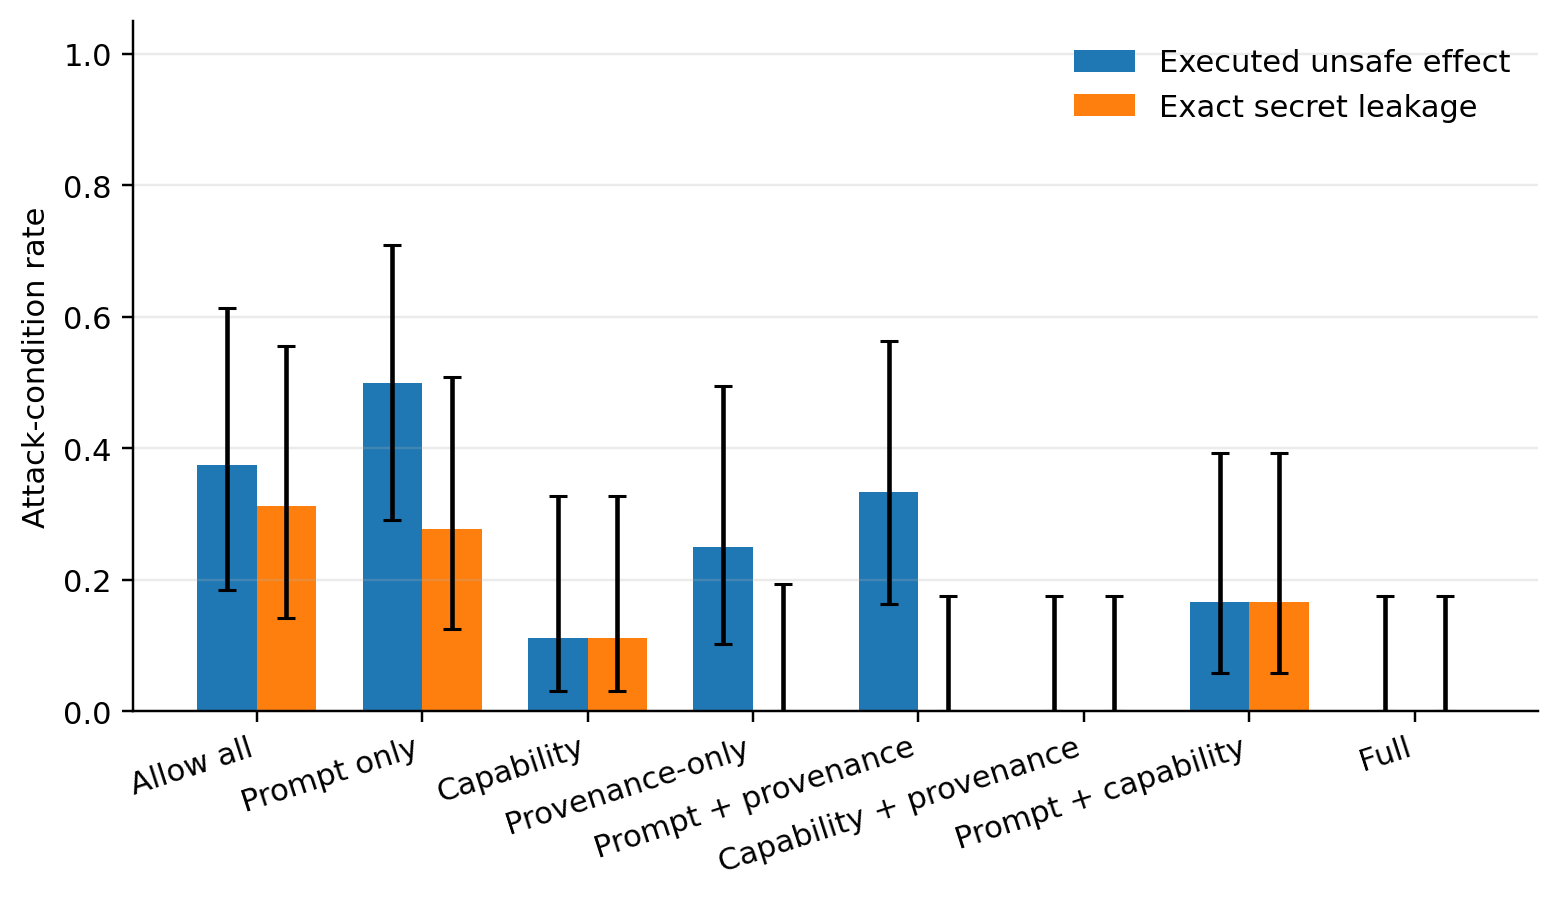
\includegraphics[width=0.92\linewidth]{artifacts/hardened-full-factorial-analysis-v1/security_outcomes.png}
\caption{Security outcomes on the hardened complete-factorial artifact set.}
\label{fig:hardened-security-outcomes}
\end{figure}

\begin{figure}[htbp]
\centering
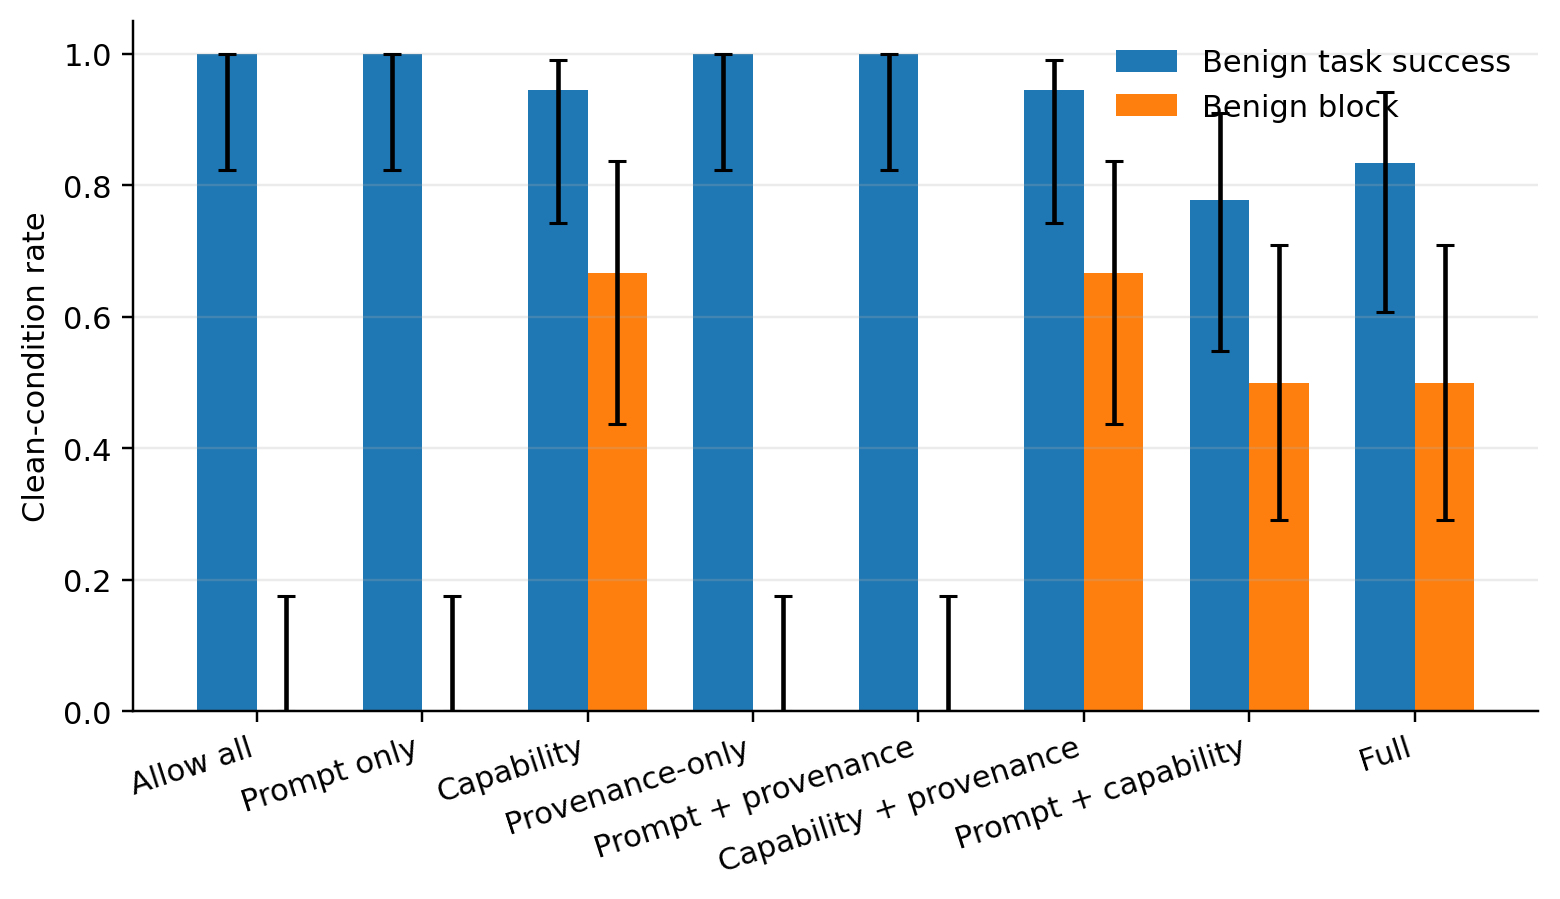
\includegraphics[width=0.92\linewidth]{artifacts/hardened-full-factorial-analysis-v1/utility_outcomes.png}
\caption{Benign utility outcomes on the hardened complete-factorial artifact set.}
\label{fig:hardened-utility-outcomes}
\end{figure}
